In order to determine which amino acids in a protein play the largest role in determining binding affinity, it is convenient to compare the binding affinity of the native protein with that of a single residue mutant.
Single point mutations with few exceptions, mutations to or from glycine, proline, and depending on the local structure possibly large amino acids, are unlikely to affect the folding of the protein \cite{illergaard2009structure,betts2003amino}.
Alanine is the most frequently occurring amino acid, appearing in both solvent exposed and buried positions \cite{chothia1976nature,rose1985hydrophobicity}, and is unlikely to disrupt the protein fold in the same way glycine or proline might \cite{klapper1977independent,betts2003amino}.
Additionally, because it lacks a charge, it does not interact electrostatically with the ligand.
These reasons make it an attractive choice as a ``control'' amino acid for mutation scanning experiments.
Mutation scanning experiments seek to identify the residues that have the largest contributions to binding affinity or ``hot spot'' residues, by identifying single residue mutants that have a significantly decreased binding affinity when mutated to alanine \cite{cunningham1989high}.
\begin{figure}[h]
\centering
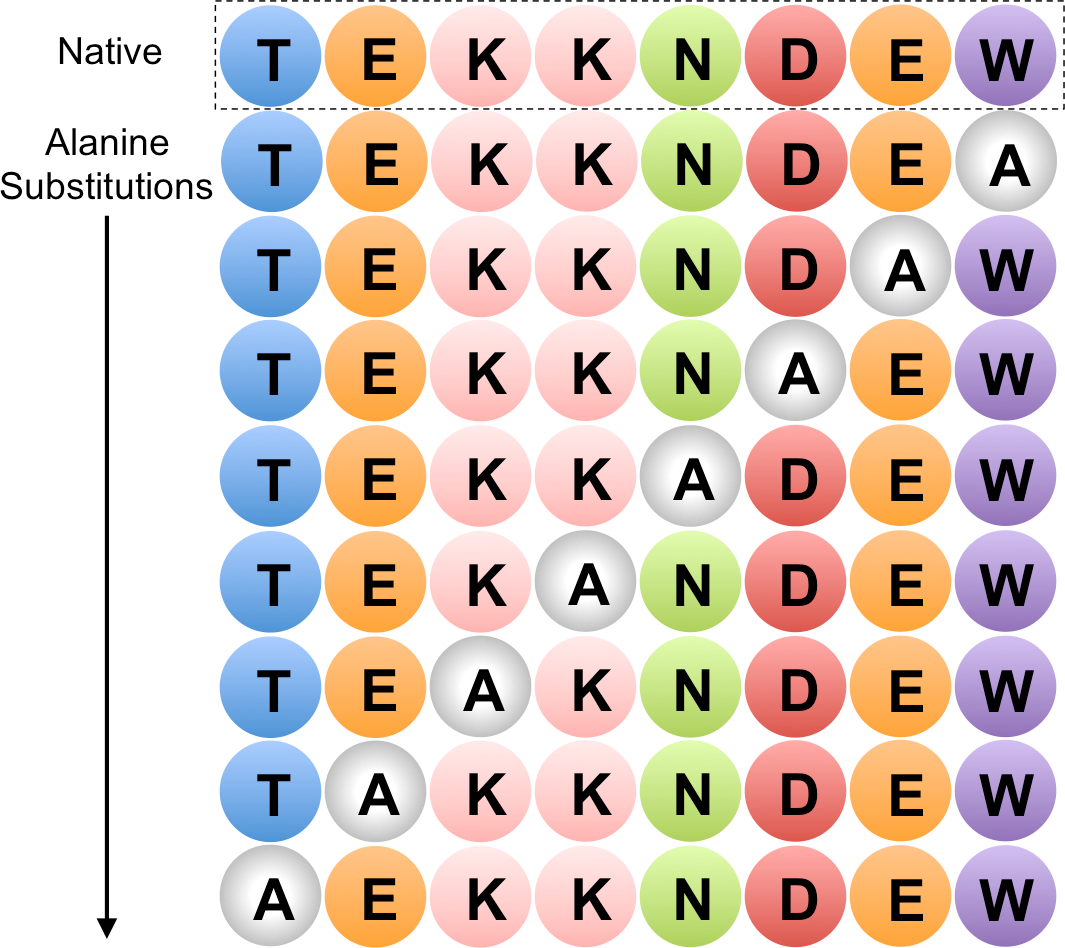
\includegraphics[width=0.5\textwidth]{figures/alanine_scan.png}
\caption{The sequences that would be evaluated during an alanine scan for Fc domain of a human IgG for streptococcal protein G.
The residues identified here were taken from the AESDB.
The native protein is represented in the top row \protect\cite{sauer1995crystal,thorn2001asedb}.}
\label{fig:alanine_scan}
\end{figure}

While generally viewed as deleterious in biology, there are a few instances in which mutations can be beneficial to an organism.
Foremost amongst these is in the immune system, where the immune system maturation response selects antibodies that have a reasonable affinity for an antigen and creates a large number of variants of these antibodies through mutation. 
The effect of this is that the body produces antibodies with increasing affinity for an antigen some time after the initial exposure \cite{griffiths1984somatic}.
In vitro affinity maturation attempts to select molecules, frequently antibodies, with high affinity for some target molecule by creating a library of bacteria, that display variants of these antibodies on their cellular surface.
This is accomplished by bacteriophage display, which provides a method of pairing the protein represented on a bacteria's surface with the genetic material contained by that bacteria \cite{smith1985filamentous}.
A bacteria is infected by a library of bacteriophages containing a large number of variants of the antibody of interest.
The phage will cause the bacteria to display its specific variant of the antibody on the bacteria surface, allowing sorting of the bacteria according to the affinity of the antigen, through affinity column purification or similar techniques.
This step greatly enriches the fraction of antibody variants binding the protein.
It is then possible to allow the bacteria to reproduce, sometimes causing more mutations to increase diversity of the antibody library and perform this affinity purification step again.
Sequential application of this affinity maturation makes it possible to identify a handful of antibody variants with high affinity from as many as $10^{6}$ different variants \cite{gram1992vitro,hawkins1992selection}.
However, the number of possible variants of the complementarity determining region (CDR) of an antibody is many orders of magnitude larger than this.

Computational mutation scanning attempts to replicate the same sort of experiment {\it in silico}.
Making the assumption that the backbone conformation is not altered by mutating a single residue to alanine, computational experiments attempt to identify hot spot residues by measuring the \ddg\ between the bound states of the native and mutated protein.
Varying cutoffs for {\it hot spot} residues are used, usually from 1.0 kcal/mol \cite{kortemme2002simple} to 4.0 kcal/mol \cite{pons1999energetic}.
Mutations at these {\it hot spot} residues tend to be strongly deleterious leading to above average conservation  \cite{hu2000conservation,lichtarge1996evolutionary}.

In this chapter we present a method of performing mutation scans to arbitrary amino acids and evaluate its performance by predicting \ddg\ binding for a number of single point mutations of hot spot residues to alanine.
We show that though the conformations of these side chains are predicted quite accurately, though, no significant correlation of free energy of binding was observed between predicted and experimental values for \ddg.

%Mutated structures were generated by truncating side chain at C\subscript{$\gamma$} \cite{massova1999computational}

% computer aided antibody design \cite{kuroda2012computer}
%\cite{moreira2007computational}

